%!TEX root = Qualificacao.tex

\section{Randomized Model Structure Selection}%
\label{sec:ramss}

% COMTEMP \todo[inline]{Coloquei o RaMSS por enquanto nesta seção, mas estou querendo colocar em um capítulo a parte. Só mencioná-lo na seção anterior como método de seleção de estrutura. No capítulo a parte colocarei uma introdução sobre métodos estatísticos e teria ainda espaço para exemplos de aplicação do RaMSS para identificação de sistemas (processos). Mai a frente abordaria o uso para identificação de controladores.} 

O método RaMSS, apresenta uma abordagem alearorizada para escolha de uma estrutura de modelo adequada por meio da amostragem de modelos de um conjunto de modelos $\mathscr{M}$. 
Introduzido por \cite{falsone2014} e aperfeiçoado em \cite{falsone2015}, o método realiza a tarefa de seleção de estrutura de maneira probabilística que, apesar do caráter aleatório, evita a busca exaustiva necessária para analisar todos os regressores do conjunto de regressores candidatos, definido por $\mathscr{R}$,
% COMTEMP \todo{tentar colocar isso (a definição do conjunto) de uma maneira mais formal (fórmula).} 
que seria necessário ao se utilizar força bruta em uma estratégia puramente Monte Carlo. 

O método procura iterativamente pelo melhor subconjunto de regressores no conjunto $\mathscr{R}$ visando maximizar a acurácia da predição do modelo segundo um índice definido. Isto é feito através de modelos candidatos, subconjuntos de $\mathscr{M}$, construídos a partir de regressores amostrados do conjunto $\mathscr{R}$ com a probabilidade de escolha dada por uma função de probabilidade estimada chamada de RIP (\textit{Regressor Inclusion Probability})
% COMTEMP \todo{passar para PT/EN}.
Uma vez escolhido um modelo candidato, este é avaliado de acordo com algum critério de desempenho e os RIP são atualizados. A cada iteração, $N_p$ modelos são tomados de $\mathscr{M}$ e índices de desempenho são calculados para a atualização dos RIP.
Estes índices são, em geral,  baseados no MSPE, MSSE ou uma combinação dos dois, e são usados para calcular um índice médio de desempenho do regressor avaliado.
% Assumindo que o $j$-ésimo regressor aparece em alguns dos  $N_p$ modelos escolhidos, x
Assumindo um conjunto $\mathscr{M}$ de $N_p = \dim(\mathscr{M})$ modelos em que alguns contêm o $j$-ésimo regressor, um índice que mensura o \textit{desempenho médio do regressor}, que pode ser usado no cálculo do RIP é definido como
\begin{align}
   \mathcal{I}_j &= \mathcal{I}_j^+ - \mathcal{I}_j^- \nonumber\\
      % &= \E[\mathcal{J}^{+}_{j}] - \E[\mathcal{J}^{-}_{j}]
      &= \E[\mathcal{J}(\Phi)|\phi_j \in \Phi] - \E[\mathcal{J}(\Phi)|\phi_j \notin \Phi],
\label{eq:desMedioReg}
\end{align}
% COMTEMP \todo{decidir aqui: usar $\Phi$ ou  $ \mathscr{R}$ -- eq. \eqref{eq:desMedioReg}.}
sendo $j = 1,\ \dots,\ m$, em que  $m = \dim{(\mathscr{R})}$ é o número de regressores considerados, $\mathcal{J}(\Phi)$ representa o vetor contendo os índices de desempenho para os modelos escolhidos, $\Phi$ é o conjunto de regressores candidatos, $\phi_j$ o $j$-ésimo regressor e $\E[\cdot]$ é o operador de esperança matemática\footnote{Caso o evento condicional tenha probabilidade nula de ocorrer, a esperança é assumida nula.}. Desta forma, o índice de desempenho $\mathcal{I}_j$ compara o desempenho médio dos modelos contendo o $j$-ésimo regressor ($ \mathcal{I}_j^+$) com o desempenho dos modelos que não contêm este mesmo regressor ($ \mathcal{I}_j^+$). 
Como em geral a esperança matemática da equação \eqref{eq:desMedioReg} não pode ser calculada de forma analítica, esta é, na prática, feita por estimação, tomando modelos do modelo universo $\mathscr{M}$ e calculando a média amostral, resultando em
\begin{equation}
   \mathcal{I}^+_j = \frac{1}{n_j^+}\sum_{i \in \mathscr{M}_j^+}\mathcal{J}^{+}_{i} \qquad \text{e} \qquad \mathcal{I}^-_j = \frac{1}{n_j^-}\sum_{i \in \mathscr{M}_j^-}\mathcal{J}^{-}_{i},
\label{eq:avgRefPerf}
\end{equation}
onde $ \mathscr{M}^+_j \subset \mathscr{M}$ e $ \mathscr{M}^+_j \subset \mathscr{M}$, representam os conjuntos de todos os modelos que, respectivamente, contêm e não contêm o $j$-ésimo regressor $\phi_j$, com $n_j^+ = \dim \mathscr{M}^+_j $ e $n_j^+ = \dim \mathscr{M}^+_j$. Os termos $\mathcal{J}^{+}_{i}$ e  $\mathcal{J}^{-}_{i}$ representam os respectivos índices de desempenho para os casos que contêm e que não contêm $\phi_j$.


% \vspace{2cm} \hrulefill

% O objetivo do algoritmo RaMSS pode ser resumido como se segue:

Assumindo que o modelo real definido por $f^*$, o qual se deseja encontrar, pertence ao conjunto de todas as possíveis estruturas (conjunto universo) $\mathscr{M}$, deve ser possível achar este modelo explorando o conjunto de modelos $\mathscr{M}$ e tomando os modelos com melhor desempenho.  O problema de se achar o modelo real em função de um índice pode ser representado por
\begin{equation}
   f^* = \argmax_{\tilde{f} \in \tilde{\mathscr{M}}} \mathcal{J}(\tilde{f}),
\label{eq:fStar}
\end{equation}
onde $ \mathcal{J}$ é algum\footnote{A definição de $\mathcal{J}$ adotada na proposta original do RaMSS é apresentada mais adiante no texto (vide eqs. \ref{eq:Jp} a \ref{eq:Jcal}). } índice de desempenho calculado para os modelos candidatos $\tilde{f}$ tomados do conjunto universo não redundante  $\tilde{\mathscr{M}} \subset{\mathscr{M}}$\footnote{Note que no conjunto universo é comum o aparecimento de modelos redundantes, oev  seja, modelos similares que não incluem termos estatisticamente relevantes. Na prática é comum que estes sejam removidos e a amostragem seja realizada em um conjunto reduzido do modelo universo, definido por $\tilde{\mathscr{M}} \subset \mathscr{M}$.}, oev   mesmo por $ \mathscr{M}$.


No sentido de achar a estrutura correta do modelo, ou seja $ f^*$, o algoritmo RaMSS amostra $N_p$ modelos de $ \mathscr{M}$, calcula o desempenho $\mathcal{J}(\tilde{f})$ para cada modelo candidato $\hat{f}_{i}$, com $i=1,\ \dots,\ N_p$ e estima a média sobre todos os modelos que envolvem o regressor $\phi_j$. Isto é feito para cada um dos $m=\dim(\mathscr{R})$ regressores do conjunto $\mathscr{R}$ de regressores candidatos.

Considerando que o índice de desempenho $\mathcal{J}$ em \eqref{eq:fStar} tenha valores no intervalo $[0,\ 1]$, i.e.  $ \mathcal{J}(\tilde{f}) \in \R : \mathcal{J}(\tilde{f}) \in [0,\ 1] $
\todo{Confirmar isso aqui}, 
% o valor esperado de $\mathcal{J}$,
seu valor esperado,
considerando $ \mathcal{P}_j$ a distribuição de probabilidade ao se escolher o regressor $\phi_j$ como variável aleatória $\Phi$ na realização de uma amostra de modelo em  $ \tilde{\mathscr{M}}$, será dado por
\begin{equation}
   \E[\mathcal{J}] = \sum_{\tilde{f}\in \tilde{\mathscr{M}}} \mathcal{J}(\tilde{f})\mathcal{P}_j(\Phi=\tilde{f})
\label{eq:espJ}
\end{equation}

Se $\mathcal{P}$ é variado sobre todas as possíveis distribuições em $\tilde{\mathscr{M}}$, o máximo de \eqref{eq:espJ} é obtido ao se concentrar toda a massa de probabilidade no modelo mais adequado. Com isso, a solução do problema de otimização pode é obtida por
\begin{equation}
   \mathcal{P}^*_j = \argmax_{\tilde{f}\in  \tilde{\mathscr{M}}} \E\left[ \mathcal{J}(\Phi)  \right]   
\label{eq:Pargmax}
\end{equation}
e é tal que $\mathcal{P}_{j}=1$. Assim, resolvendo \eqref{eq:Pargmax} seleciona-se o modelo mais adequado, ou modelo real $f^*$, com a mesma solução de \eqref{eq:fStar}.

O método RaMSS estima $\mathcal{P}_{j}$ e, consequentemente, o melhor modelo como se segue. A cada iteração, $N_p$ modelos candidatos são montados a partir de $m$ regressores candidatos. A escolha de cada regressor $\phi_j$ componente de um modelo candidato é feita a partir de um processo de Bernoulli, por uma variável aleatória associada a cada regressor  $\phi_j$ tal que
\begin{equation}
   \rho \approx \text{Be}(\mu_j),
\label{eq:bernulli}
\end{equation}
onde possíveis resultados são: 1, com probabilidade (de sucesso) $\mu_j$ de ocorrer; e 0, com probabilidade $(1-\mu_j)$; sendo $\mu_j \in [0,\ 1]$,  com $ j=1, \dots, m$ e $m$ o número de regressores candidatos. 
Caso $\rho=1$, o regressor  $\phi_j$ estará presente no modelo candidato construído, caso contrário, não. 

Assume-se que variáveis aleatórias $\rho_j$ são independentes\footnote{Apesar de existirem resultados na literatura \citep{bianchi2016} sugerindo que uma abordagem utilizando distribuição Bernoulli condicionada e multivariada pode resultar em melhorias na acurácia do processo de seleção de modelos, um procedimento inicial adotado neste trabalho considera independência.} e define-se um vetor $\bm{\mu} = [\mu_1,\ \mu_2,\ \dots,\ \mu_m]^T$ como o vetor de \textit{Probabilidade de Inclusão de Regressor} (RIP). Note que o RIP, ou $\vmu$ é quem dita a distribuição de probabilidade  $ \mathcal{P}_j$ sobre os modelos em $\tilde{\mathscr{M}}$ (ou $\mathscr{M}$), ou seja, dado um $\bm{\mu}$ conhecido, a probabilidade de se obter um modelo de estrutura $\tilde{f}$ em qualquer subconjunto de $n_\theta$ regressores será
\begin{equation}
   \mathcal{P}_j(\tilde{f}) = \prod_{j:\phi_j \in \tilde{f}}^{n_{\theta}} \mu_j \prod_{j:\phi_j \notin \tilde{f}}^{m-n_{\theta}} (1-\mu_j),
\label{eq:distProbf_til}
\end{equation}
para qualquer $ \tilde{f} \in \tilde{\mathscr{M}}$.

O procedimento é executado de modo que a cada iteração os regressores são escolhidos de acordo com o processo de Bernoulli, onde a probablilidade de escolha $\mu_j$ de cada regressor $\phi_j$ é representada pelo vetor de RIP. O vetor de RIP, $\bm{\mu}$ é refinado por sucessivas iterações de uma regra de atualização definida como
\begin{equation}
   \mu_j(i+1) = \mu_j(i) + \gamma \mathcal{I}_j,
\label{eq:RIPupdate}
\end{equation}
onde $\gamma$ é um parâmetro de projeto, $I_j$ o índice de desempenho definido em \eqref{eq:desMedioReg} e $i$ o índice da iteração do algoritmo.

% \vspace{2cm} \hrulefill

Depois de algumas iterações é esperado que os desempenhos médios dos modelos que contém os regressores certos fiquem significantemente maiores que os que não contém, fazendo com que os regressores ``corretos'' sejam mais prováveis de serem incluídos no modelo final. O método não garante que $ \bm{\mu}$ será limitado. Para evitar que os valores do RIP cresçam, ou decresçam indefinidamente, uma saturação dos elementos em uma faixa com valor mínimo maior ou igual a 0, e máxima, menor ou igual a 1, é aplicada pelo algoritmo.

O parâmetro de projeto $\gamma$, de  \eqref{eq:RIPupdate} é escolhido de forma a controlar a velocidade de convergência. Valores maiores tendem a levar a uma convergência mais rápida mas pode também levar a não convergência do método. Para lidar com este problema de convergência, \cite{falsone2015} propõem um parâmetro adaptativo, dado por
\begin{equation}
   \gamma = \frac{1}{10(\mathcal{J}_{\max}- \bar{\mathcal{J}}) + 0.1}, 
\label{eq:gamma}
\end{equation}
onde $\mathcal{J}_{\max}$ representa o índice de desempenho do melhor modelo e $\bar{\mathcal{J}}$ representa o índice de desempenho médio na iteração corrente.
A proposta do passo adaptativo é de que, se $\bar{\mathcal{J}}$ está longe do melhor índice de desempenho, $\gamma$ é feito pequeno de modo a compensar a grande variância provável daquela população de modelos. Porém, se  $\bar{\mathcal{J}}$ é próximo de $\mathcal{J}_{\max}$, os modelos amostrados têm baixa variância de desempenho, o que indica que o RIP deve ser atualizado em maior valor.

O método RaMSS, como apresentado originalmente pelos autores, utiliza como base para o cálculo do índice de desmpenho médio $\mathcal{J}$, grandezas relacionadas ao MSPE e ao MSSE, definidos na seção \ref{sec:model_validation}. O índice de desempenho médio é calculado como um valor exponencial destes índices ponderados por um ganho $K$, utilizado como parâmetro de projeto. Desta forma tem-se,
\begin{align}
  \mathcal{J}_p = e^{-K\cdot MSPE}, \label{eq:Jp} \\
  \mathcal{J}_s = e^{-K\cdot MSSE}. \label{eq:Js}
\end{align}
Note que $J_p$ e $J_s$ terão valores no intervalo $[0 \ 1]$, onde valores próximos a 1 correspondem a um melhor desempenho, e próximos a 0, a piores desempenhos.

O valor final de $\mathcal{J}$ é calculado como
\begin{equation}
  \mathcal{J} = \alpha \mathcal{J}_s + (1-\alpha)\mathcal{J}_p
\label{eq:Jcal}
\end{equation}
onde $\alpha \in [0 \ 1]$ é um parâmetro definido pelo projetista. O parâmetro $K$ define a sensibilidade do índice de desempenho, onde a diferença entre modelos é amplificada para valores maiores de $K$.

% COMTEMP \todo[inline, color=red]{Continuar aqui!??}

% TODO: [DONE] {Colocar aqui sobre $\mathcal{J}$, como é definido, etc.}

Passadas algumas iterações o espera-se que vetor de RIP, $\bm{\mu}$, convirja para uma distribuição de equilíbrio. O modelo final será o modelo correto esperado do sistema e será composto pelos regressores associados aos RIP com valores maiores que certo limiar definido pelo projetista. Assumindo-se que o modelo real $f^* \in \tilde{\mathscr{M}}$, este limiar em geral é ajustado para um valor próximo a 1.

O pseudo-código para o método RaMSS descrito é apresentado no Algorithm \ref{alg:RaMSS}. Na sequência é apresentado  um exemplo para identificação de sistema utilizando o  método.
    % \For(\tcp*[f]{Start Policy Improvement}){each $\vx_k \in \Omega_k$}

\begin{algorithm}[H]
  \caption{RaMSS algorithm}\label{alg:RaMSS}
  $\bm{y},N_p,m,\mu_{\min},\mu_{\max},K,\Phi=\{\phi_{1},\dots,\phi_{m}\}$ \\
  \While{$iter < iter_{\max}$} 
   {
     $ \bm{\mu} \gets \bm{\mu}_0$
     \For(\tcp*[f]{Model Sampling}){$i=1:N_p$}
      {
         $\tau \gets 0$ \\
         $\bm{\psi}(k) \gets [\ ]$ \tcp*[f]{Initialize model} \\
         \For{$i=1:m$}
         {
           $r_j \gets \text{Be}(\mu_j)$ \tcp*[f]{Sample from a Bernoulli distribution}\\
            \If{$r_j = 1$}
            {
            $\bm{\psi}(k) \gets \begin{bmatrix} \bm{\psi}^T(k) & \phi_j \end{bmatrix}^T $ \\
            $\tau \gets \tau + 1$ \\
            }
         }
         \For{$h=1:\tau$}
         {
           $\tilde{\bm{\psi}}(k) \gets \text{non-redundant}(\bm{\psi(k)})$ \tcp*[f]{Remove redundant terms}\\
         }
         $\hat{\bm{y}} \gets \text{Predict}(\tilde{\bm{\psi}}(k))$ \\
         $\mathcal{J}_i \gets e^{-K\cdot MSPE(\bm{y},\bm{\hat{y}})} $
      }
      \For(\tcp*[f]{RIP Update}){$j=1:m$}
      {
         $\mathcal{J}^{+} \gets 0$; $ \mathcal{J}^{-}$; $n^{+} \gets 0$; $n^{-} \gets 0$; \\
         \For{$i=1:N_p$}
         {
            \If{$\phi_j(k) \in \tilde{\bm{\psi}}(k)$}
            {
               $\mathcal{J}^{+} \gets \mathcal{J}^{+} + \mathcal{J}_i$ \\
               $n^{+} \gets n^{+} + 1$
            } \Else
            {
               $\mathcal{J}^{-} \gets \mathcal{J}^{-} + \mathcal{J}_i$ \\
               $n^{-} \gets n^{-} + 1$
            }
            $\mathcal{I}_j \gets \left( \frac{\mathcal{J}^{+}}{\max(n^+,1)} \frac{\mathcal{J}^{-}}{\max(n^-,1)} \right) $ \\
         $\mu_j \gets \mu_j + \gamma \mathcal{I}_j$ \\
         $\mu_j \gets \max \left( \min(\mu_j, \mu_{\max}), \mu_{\min} \right) $ \\
         }
      }
   }
\end{algorithm}%[H]

\begin{exmp}[Idendificação de um modelo não-linear utilizando o RaMSS]
  \label{ex:varHeater}
  Como exemplo ilustrativo da utilização do algoritmo RaMSS na escolha de estrutura e identificação de sistemas é usado um modelo de um pequeno aquecedor elétrico, com dissipação variável. A variação da dissipação é resultado do acionamento de um ventilador. O sinal de entrada é a tensão elétrica aplicada ao aquecedor e a saída é o sinal amplificado de um termopar. Mais detalhes sobre este modelo podem ser encontrados em \citep{aguirre2015}, seção 16.6.

  \begin{figure}[H]
    \centering
    
\includegraphics{./Figs/s.heater.var.dissip_RIPs.eps}
    \caption{Evolução dos RIPs durante as iterações do algoritmo RaMSS.}
    % COMTEMP \todo[inline]{Colocar linha de \textit{threshold} na ref{fig:RIPs1}? Mudar cores. Tentar mudar nome dos regressores (índices). Mas com certeza, mudar nomes de y para u.}
    \label{fig:RIPs1}
  \end{figure}

  \begin{figure}[H]
    \centering
    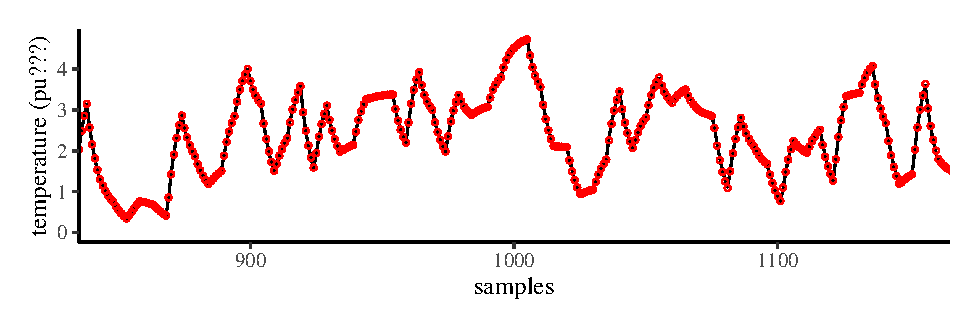
\includegraphics{./Figs/s.heater.var.dissip_train_val_data.eps}
    \caption{Resposta temporal para os dados de amostrados (preto tracejado -\ -), treinamento (círculos vermelhos $\color{red} \circ$), até a iteração 1000, e de validação (vermelho contínuo) a partir da milésima iteração. Para melhor visualização apenas as iterações de 850 a 1150 são mostradas. }
    \label{fig:}
    % \todo[color=orange, inline]{\textbf{LAA: } Não colocar dados de treinamento, somente validação. Deixar claro que foi utilizado free-run simulation.}
    % \todo[inline]{Corrigir axis labels}
  \end{figure}

\end{exmp}

